\scanpage{32}\mspage{31}

Si $A\in F\setminus G$, $A\cap B$ est réunion de strates de $F$. \deleted{\unsure{Reste}} reste \unsure{à|:} voir que une strate \inserted{\unsure{$G$|$\in$|e}} de $F$ est réunion de strates de $F'$. Soit $A$ cette strate de $F$. \deleted{\unsure{On|les|le}}
\[
 \deleted{A=\bigcup_{\substack{B\in F\\B\leq F}}B^\circ}
\]
Si $A\notin G'$, \unsure{donc|alors} $A\in F\setminus G'\subset F'$, et on gagne. Si $A\in G$, alors (comme $G'\preceq G$) $A$ est réunion de strates de $G'$, qui sont des strates de $F'$, et on gagne encore.

% slanted
\margin{Ultra faux}
\uline{Corollaire} Le \deleted{raffinement}\inserted{subdivision} précédente $F'$ de $F$ est caractérisée par \inserted{chacune} des \unsure{pr.|pro.} propriétés équivalentes suivantes~:

\deleted{a) Pour toute subdivision $F''$ de $F$ qui induit $G'$ sur $G$, on a $F''\preceq F'$ -- i.e. $F'$ est \deleted{\uline{maximal}}\inserted{un plus grand \unsure{élémt|élément|élt}}, pour $\preceq^{*}$, \unsure{dans|pour} l'ens des subdivisions de $F$ qui induisent $G'$ sur $G$.}
% slanted
\margin{$*$ ou pour $\ll$, cela revient au $=$ parmi des subdivisions d'une $=$ $F$}
% slanted; live state preferred, whole-note cancellation explicitly retained as an alternative.
\margin{\unsure{\figure{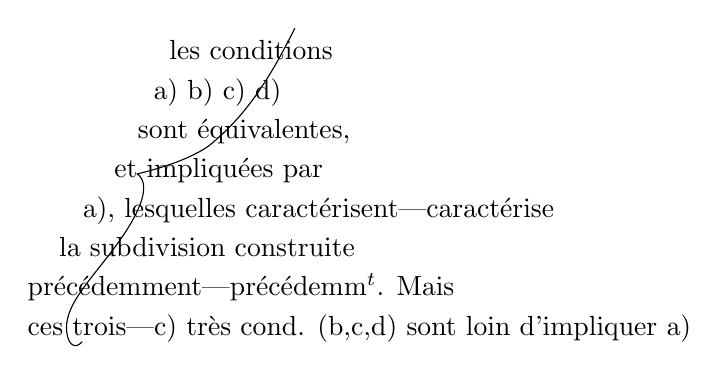
\begin{tikzpicture}[x=1mm,y=1mm,
 every node/.style={anchor=base west,inner sep=0pt}]
 \node at (18,0) {les conditions};
 \node at (16,-5) {\deleted{\unsure{a)}} b) c) d)};
 \node at (14,-10) {sont équivalentes,};
 \node at (11,-15) {\unsure{et} \uline{impliquées} par};
 \node at (7,-20) {a), lesquelles \unsure{caractérisent|caractérise}};
 \node at (4,-25) {la subdivision construite};
 \node at (0,-30) {\unsure{précédemment|précédemm$^{t}$}. Mais};
 \node at (0,-35) {\unsure{ces trois|c) très} \unsure{cond.} (b,c,d) \unsure{sont} \unsure{loin} d'impliquer a)};
 \draw (34,4)
  .. controls (31,-2) and (28,-7) .. (23,-11)
  .. controls (20,-13) and (16,-14) .. (14,-14.5)
  .. controls (16,-16) and (14,-20) .. (11,-24)
  .. controls (8,-28) and (5,-31) .. (5,-34)
  .. controls (5,-36) and (6,-37) .. (7,-35.8);
\end{tikzpicture}}|\deleted{les conditions \deleted{\unsure{a)}} b) c) d) sont équivalentes, \unsure{et} \uline{impliquées} par a), lesquelles \unsure{caractérisent|caractérise} la subdivision construite \unsure{précédemment|précédemm$^{t}$}. Mais \unsure{ces trois|c) très} \unsure{cond.} (b,c,d) \unsure{sont} \unsure{loin} d'impliquer a)}}}

% Small additional a)-like label above the end of application, attachment uncertain.
b) L'application \inserted{\unsure{a)}} can. associée à $F'\preceq F$
\[
 \varphi:F'\longrightarrow F
\]
induit une bijection
\[
 F'\setminus G'\xrightarrow{\sim}F\setminus G.
\]
\margin{\figure{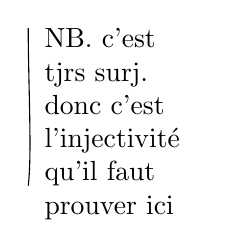
\begin{tikzpicture}[x=1mm,y=1mm]
 \draw (0,0) .. controls (0,-7) and (0.5,-16) .. (0,-20);
 \node[anchor=north west,inner sep=0pt,align=left,text width=20mm] at (2,0) {NB. c'est tjrs surj. donc c'est l'\uline{injectivité} qu'il faut prouver ici};
\end{tikzpicture}}}

c) \deleted{Les strates ouvertes de $F'$ qui ne \unsure{sont}} \inserted{$\forall A\in F\setminus G$, $A^\circ$ est une \unsure{str.te|strate|str.} ouverte} de $F'$.

d) $F'\supset F\setminus G$, i.e. $\forall A\in F\setminus G$, on a $A\in F'$.

\uline{Dém} On va prouver p. ex
\[
 \text{d)}\Longrightarrow\text{b)}\Longrightarrow\text{c)}\Longrightarrow\text{a)}\Longrightarrow\text{d)}
\]
\deleted{\uline{\unsure{Dém}}} $\text{d)}\Rightarrow\text{b)}$ Si $(F\setminus G)\subset F'$, alors $\varphi\mid F\setminus G$ est l'\deleted{\unsure{identité}}inclusion \deleted{(trivial)} \inserted{can. $F\setminus G\hookrightarrow F$}, \deleted{donc} donc il reste à prouver
\[
 F\setminus G=F'\setminus G'.
\]
